\section{Capítulo 4: Análisis de Resultados y Juicio de Ingeniería}

\subsection{Resultados de Verificación (Pruebas de Software)}
% Guia: resultados de pruebas unitarias, de integracion, de sistema y de cobertura.
La verificación del sistema de Thary se llevó a cabo mediante pruebas automatizadas escritas con \textit{pytest}, ya explicadas en la Sección \ref{sec:verificacion_validacion}. Los resultados de estas pruebas se obtuvieron ejecutando el comando \texttt{pytest tests/ -v} en la terminal.

\begin{figure}[H]
    \centering
    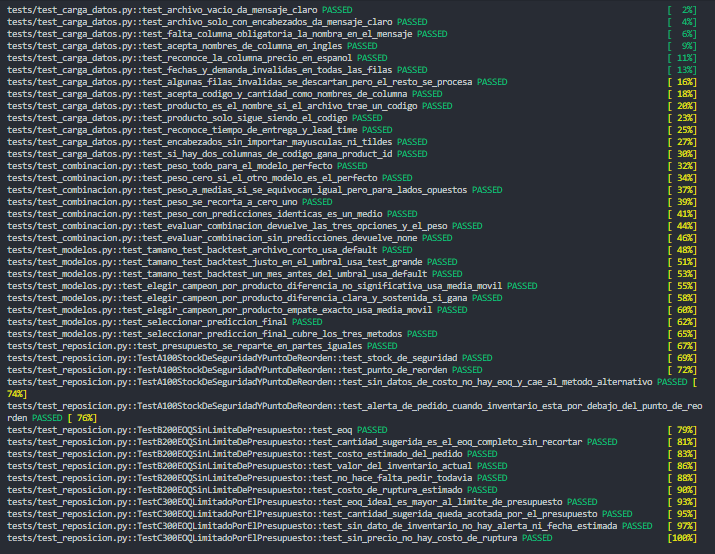
\includegraphics[width=\textwidth]{templatefigures/pytest_resultados_verbose}
    \caption{Ejecución detallada de la suite de pruebas mediante \texttt{pytest tests/ -v}, mostrando cada prueba individual.}
    \label{fig:pytest_verbose}
\end{figure}

\begin{table}[H]
    \centering
    \caption{Resultados de la suite de pruebas automatizadas por archivo.}
    \label{tab:resultados_pruebas}
    \renewcommand{\arraystretch}{1.3}
    \begin{tabularx}{\textwidth}{|l|X|c|}
    \hline
    \textbf{Archivo} & \textbf{Componente verificado} & \textbf{Resultado} \\
    \hline
    \texttt{test\_carga\_datos.py} & Carga y limpieza de datos, incluyendo el reconocimiento de columnas heterogeneas & 13/13 exitosas \\
    \hline
    \texttt{test\_combinacion.py} & Combinación de pronósticos & 7/7 exitosas \\
    \hline
    \texttt{test\_modelos.py} & Selección del modelo campeón y prueba Diebold-Mariano & 8/8 exitosas \\
    \hline
    \texttt{test\_reposicion.py} & Calculo de reposición (stock de seguridad, punto de reorden, EOQ, costo de ruptura) & 15/15 exitosas \\
    \hline
    \textbf{Total} & & \textbf{43/43 exitosas} \\
    \hline
    \end{tabularx}
\end{table}

\begin{figure}[H]
    \centering
    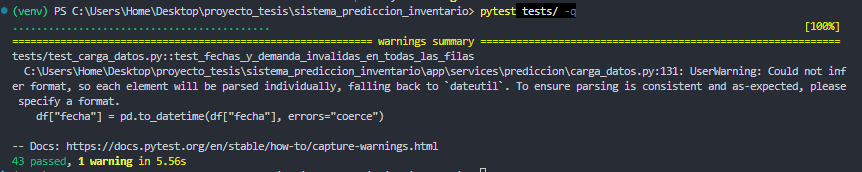
\includegraphics[width=0.8\textwidth]{templatefigures/pytest_resultados_resumen}
    \caption{Resumen final de la ejecución mediante \texttt{pytest tests/ -q}.}
    \label{fig:pytest_resumen}
\end{figure}

Como se puede ver en la Fig. \ref{fig:pytest_verbose}, la Tabla \ref{tab:resultados_pruebas} y la Fig. \ref{fig:pytest_resumen}, las 43 pruebas se ejecutaron correctamente en un tiempo de 5.56 segundos. Se registro una única advertencia (\textit{warning}) relacionada con el formato de fechas de pandas al procesar un archivo de prueba con fechas invalidas a proposito, sin que esto afecte el resultado de la prueba.


Se detecto un bug menor en el que la columna de "Precio" en español no era reconocida por el sistema a pesar de que la interfaz de carga la anunciaba como aceptada. Se arreglo el problema y dentro de \texttt{test\_carga\_datos.py} se incluyó la prueba \texttt{test\_reconoce\_la\_columna\_precio\_en\_espanol}, cuyo resultado exitoso confirma que la corrección aplicada sigue vigente.

El mecanismo de reconocimiento de columnas se reforzó con seis pruebas adicionales que verifican, entre otros casos: que el sistema ignore mayusculas y tildes en los encabezados, que resuelva correctamente la ambiguedad entre "Producto" como código o como nombre del producto (según si el archivo ya trae una columna de código clara), y que priorice la columna correcta cuando un archivo trae más de un candidato para el mismo destino (por ejemplo, un "Id" de transaccion junto a un "Product\_ID" real).
Además de las pruebas automáticas, se revisó de forma manual que la función principal de Thary se hiciera bien de principio a fin. Es decir, que el sistema dejara cargar un archivo, procesarlo, mostrar los resultados y confirmar un pedido sin errores. Las etapas de segmentación de productos, construcción de variables, y las rutas y autenticación de la aplicación web no tienen pruebas automáticas. Esto se reconoce como una limitación de la revisión.

\subsection{Resultados de la Validación del Modelo de Predicción}
% Resultados de la validacion cruzada temporal y del holdout final: metricas
% por modelo, consistencia entre folds, y verificacion del criterio de
% aceptacion definido en la Seccion 3.4.3.
A continuación, se presentan los resultados obtenidos en la validación del sistema Thary. Estos resultados se obtuvieron luego de aplicar la estrategia de validación ya definida anteriormente, sobre el historial real de consumo de 856 productos (medicamentos) del año 2021 - 2022 en la Clínica Nuestra Señora de los remedios. 

Las métricas obtenidas al evaluar los tres modelos candidatos, junto con el método de selección de modelo por producto. Todo esto sobre el último periodo de prueba disponible, que corresponde al trimestre abril-junio de 2022, con seis meses de entrenamiento previo.

\begin{table}[H]
    \centering
    \caption{Métricas del holdout final por modelo.}
    \label{tab:resultados_holdout}
    \renewcommand{\arraystretch}{1.3}
    \begin{tabularx}{\textwidth}{|X|c|c|c|c|c|}
    \hline
    \textbf{Modelo} & \textbf{MAE} & \textbf{RMSE} & \textbf{Mediana Error} & \textbf{MAPE (\%)} & \textbf{WAPE (\%)} \\
    \hline
    Media Móvil (3 meses) & 48.79 & 243.65 & 5.33 & 80.32 & 23.86 \\
    \hline
    Regresión Lineal      & 56.43 & 276.41 & 5.25 & 95.30 & 27.60 \\
    \hline
    XGBoost (log1p)       & 50.59 & 254.82 & 3.53 & 65.12 & 24.74 \\
    \hline
    \textbf{Sistema final (selección por producto)} & \textbf{48.47} & \textbf{243.55} & --- & \textbf{79.33} & \textbf{23.71} \\
    \hline
    \end{tabularx}
\end{table}

\begin{figure}[H]
    \centering
    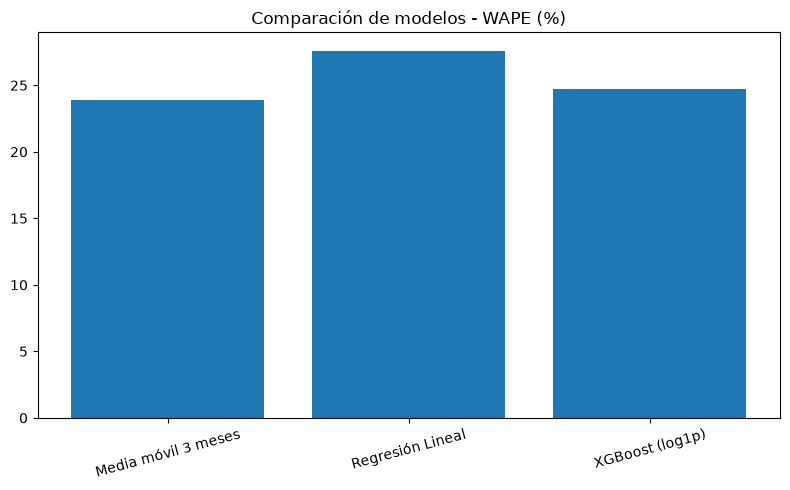
\includegraphics[width=0.75\textwidth]{templatefigures/comparacion_WAPE_porcentaje}
    \caption{Comparación de WAPE entre los tres modelos candidatos (holdout final).}
    \label{fig:comparacion_wape}
\end{figure}

\subsubsection{Consistencia mediante validación cruzada temporal}

Después de obtener los resultados anteriores, se propuso el uso de una validación cruzada para descartar que el resultado obtenido dependiera de las condiciones y particularidades de un único periodo de prueba.

La idea principal, es probar el modelo varias veces simulando estar en un mes distinto al pasado, para poder evaluar si acierta de forma consistente y no solo una vez por casualidad. Para poder predecir un mes, solo se puede usar los meses que vinieron antes, no se pueden usar los datos que serían "Futuros", porque queremos simular un escenario real, y en ese caso, no se tendría esa información.

\begin{enumerate}
    \item Prueba 1 (Fold 1): Es el más antiguo, se le enseña al modelo con los 4 meses previos a febrero de 2022, y se hace que el sistema adivine febrero, marzo y abril de 2022. Se compara lo que adivino contra los resultados reales de esos meses y se registra que tan grande fue el error.
    \item Prueba 2 (Fold 2): En esta segunda prueba o Fold, se le enseña al modelo con 5 meses en vez de 4, es decir, los meses previos a marzo de 2022, y se le pide que prediga marzo, abril y mayo de 2022, una vez más, se compara y se registra el error.
    \item Prueba 3 (Fold 3): Por último, se le enseña al modelo con los 6 meses previos a abril de 2022 y se le solicita al sistema que prediga abril, mayo y junio de 2022, se compara y, una vez más, se registra el error. Este último fold corresponde al mismo holdout final presentado en la Tabla \ref{tab:resultados_holdout}.
\end{enumerate}


Dicha validación cruzada temporal se implementó en el sistema en el archivo \texttt{app/services/prediccion/validacion.py}.

\Needspace{10\baselineskip}
\captionof{listing}{Constantes y función \texttt{\_armar\_folds} de la validación cruzada temporal.}\label{lst:validacion_folds}
\begin{minted}{python}
TEST_SIZE_MESES = 3
MIN_TRAIN_MESES = 3
MAX_FOLDS = 3


def _armar_folds(meses_ordenados):
    n = len(meses_ordenados)
    folds = []
    fin_test = n
    while len(folds) < MAX_FOLDS:
        inicio_test = fin_test - TEST_SIZE_MESES
        if inicio_test < MIN_TRAIN_MESES:
            break
        folds.append((meses_ordenados[:inicio_test], meses_ordenados[inicio_test:fin_test]))
        fin_test -= 1
    folds.reverse()
    return folds
\end{minted}

Se definen tres constantes, \texttt{TEST\_SIZE\_MESES}, \texttt{MIN\_TRAIN\_MESES} y \texttt{MAX\_FOLDS}, que definen el tamaño de la ventana de prueba, el tamaño mínimo de la ventana de entrenamiento y el número máximo de folds a generar, respectivamente.


Se arma la función que genera las particiones \texttt{\_armar\_folds}, esta recibe una lista de todos los meses disponibles organizados cronologicamente. Se define el fold más reciente, es decir, los últimos meses disponibles \texttt{TEST\_SIZE\_MESES}. En cada iteracion se retrocede el punto de corte de un mes hacia atrás en el tiempo, de esta manera, se crea un nuevo Fold cuyo entrenamiento crece en un mes respecto al anterior. Este proceso se repite hasta completar \texttt{MAX\_FOLDS}, o hasta que ya no quede suficiente historial y el tamaño de la ventana de entrenamiento sea menor a \texttt{MIN\_TRAIN\_MESES} meses de entrenamiento.  

Al finalizar, los folds se ordenan en orden cronológico del más antiguo al más nuevo antes de ser devueltos.

Al ya tener los folds organizados, el sistema entrena nuevamente los tres modelos candidatos, y selecciona el mejor modelo por producto, evaluando el resultado bajo la etiqueta de "Sistema final". Es decir, es la estrategia que usa Thary para predecir el consumo, en vez de escoger uno solo, para cada producto, el sistema entrena los 3 modelos y selecciona el que se equivocó menos con ese producto en particular.

Un aspecto importante es que, la elección de qué modelo usar para cada producto se hace solo con los datos de entrenamiento, antes de ver los datos de prueba. Esto demuestra que no se está "haciendo trampa", ya que el sistema no tiene acceso a los datos de prueba, y por lo tanto, no puede "aprender" de ellos.

Aun así, solo esto no basta para confiar en el resultado, ya que aun si el sistema está eligiendo el modelo de forma honesta, un único experimento podría haber salido bien por casualidad y no porque el sistema de verdad sea bueno.


Es por eso que la validación cruzada aportó valor al sistema, ya que al repetir este mismo proceso (entrenamiento, elección del modelo y evaluación) en diferentes periodos de prueba, se confirma que el resultado obtenido en el holdout final no fue un resultado aislado, sino que se repite de forma consistente en distintos periodos de prueba.

En la siguiente tabla se describen el promedio y la desviación estándar de las métricas obtenidas en cada fold, para cada modelo candidato y el sistema final:

\begin{table}[H]
    \centering
    \caption{Resumen de la validación cruzada temporal (promedio $\pm$ desviación, 3 folds).}
    \label{tab:resumen_cv}
    \renewcommand{\arraystretch}{1.3}
    \begin{tabularx}{\textwidth}{|X|c|c|c|c|}
    \hline
    \textbf{Modelo} & \textbf{MAE} & \textbf{RMSE} & \textbf{MAPE (\%)} & \textbf{WAPE (\%)} \\
    \hline
    Media Móvil        & 44.27 $\pm$ 3.70  & 200.82 $\pm$ 41.31 & 82.38 $\pm$ 1.85  & 22.31 $\pm$ 1.29 \\
    \hline
    Regresión Lineal   & 58.13 $\pm$ 2.21  & 270.35 $\pm$ 6.32  & 106.24 $\pm$ 10.64 & 29.38 $\pm$ 1.84 \\
    \hline
    XGBoost            & 46.58 $\pm$ 3.46  & 223.64 $\pm$ 31.40 & 64.93 $\pm$ 2.25  & 23.48 $\pm$ 1.15 \\
    \hline
    \textbf{Sistema final} & \textbf{43.42 $\pm$ 3.77} & \textbf{190.50 $\pm$ 40.63} & \textbf{81.13 $\pm$ 1.56} & \textbf{21.88 $\pm$ 1.34} \\
    \hline
    \end{tabularx}
\end{table}

De la tabla se puede observar que:

\begin{itemize}
    \item El sistema final es el que obtiene el mejor promedio en las cuatro
    métricas evaluadas. En cuanto a la estabilidad entre folds, presenta la
    menor desviación estándar en RMSE y MAPE, aunque una desviación ligeramente
    mayor a la de la Media Móvil en MAE y WAPE. Esto es significativo, porque
    demuestra que vale la pena la complejidad de elegir un modelo distinto para
    cada producto: el sistema final es consistentemente más preciso en promedio,
    aunque su ventaja en estabilidad no se cumple de forma uniforme en las
    cuatro métricas.
    \item La media móvil es el segundo mejor modelo, seguido por XGBoost y finalmente la regresión lineal. Cuando se comparan los tres modelos candidatos de forma individual, la media móvil es la que obtiene un mejor MAE, RMSE y WAPE, mientras que solo XGBoost la supera en MAPE. El hecho de que ninguno de los dos modelos más sofisticados domine de forma general sobre la línea base avala la decisión de seleccionar un modelo distinto por producto, ya que no existe un único modelo que sea el mejor en todos los casos.
    \item La Regresión Lineal es la que tiene los peores resultados en las cuatro métricas, además de que su MAPE es el que más varía entre los 3 folds. Esto es coherente con la tendencia de este modelo a sobreestimar los productos de alta demanda, observada previamente en el análisis de dispersión entre modelos, lo que ayuda a explicar por que su error resulta más alto que el de los otros dos modelos.
    \item Finalmente, se observa que la efectividad del sistema final no se debe solamente a "elegir el mejor modelo en general", que en este caso seria la media móvil, sino a elegir un modelo distinto para cada producto. En caso de haber elegido media móvil para todos los productos, el error hubiera sido de 22.31\% de WAPE, mientras que al elegir el mejor modelo por producto, validado mediante la prueba de Diebold-Mariano, el error se reduce a 21.88\%
\end{itemize}

\subsection{Resultados de Validación (Evaluación del Usuario)}
% Guia: evaluacion con usuarios reales: metodo, metricas y resultados.
Para validar la usabilidad de Thary, se siguió el plan de validación ya definido. La realización de la retroalimentación fue hecha por el desarrollador del sistema y por una persona encargada de la gestión de inventarios en el dominio de salud, esto con el fin de obtener una perspectiva externa a la del equipo de desarrollo.

Para un usuario registrado como administrador el flujo del sistema se pudo completar sin dificultad e incluyó: inicio de sesión, carga y procesamiento del historial de consumo, consulta del dashboard de demanda pronosticada, del estado del inventario, del presupuesto y del calendario de pedidos y confirmación (y reversión) de un pedido sugerido. 

Una vez completado todo el proceso, la interfaz fue percibida como intuitiva y fácil de usar, no fue necesario que existiera alguna explicación adicional más allá de la que la propia interfaz del sistema proporcionaba a la hora de completar cada una de las tareas.

Como resultado de esta validación, se aportó una mejora de la usabilidad del sistema. El gestor de inventario que probó el sistema sugirió una mejora concreta: incorporar  una plantilla de archivo CSV descargable desde la propia interfaz que le sirviera a los usuarios de guía sobre el formato y columnas esperadas antes de cargar su propio histórico de consumo.  Esta sugerencia se identificó como valiosa porque, si bien Thary ya estaba diseñado para aceptar distintas variantes de nombres de columna, y en la pantalla de carga se incluye un manual con los nombres de las columnas, la incorporación de una plantilla facilita aún más este proceso al mostrarle al usuario el formato esperado antes de que intente cargar su propio archivo.

Esta sugerencia se implementó en el sistema incluyendo el archivo \texttt{plantilla\_thary.csv}, el cual está disponible para descarga desde la interfaz de carga de archivo.

Se reconoce que esta validación tuvo un carácter informal y con un número reducido de participantes (dos personas), no obstante, al incluir a una persona con experiencia real en gestión de inventario en el dominio de salud, la retroalimentación obtenida se considera representativa del tipo de usuario final para el cual Thary fue diseñado, y se identifica como una línea de trabajo futuro la realización de una validación de usabilidad más extensa, con un número mayor de participantes.


\subsection{Evaluación de la Seguridad y Estándares}
% Guia: resultados del analisis de seguridad y nivel de cumplimiento de los
% estandares declarados en el capitulo 2.
La seguridad de Thary fue evaluada en base al rendimiento que tienen las mitigaciones implementadas en el sistema frente a las amenazas identificadas mediante el modelo STRIDE.

\subsubsection{Resultados del análisis de amenazas (STRIDE)}

En la siguiente tabla se pueden ver los resultados del estado de cada una de las partes de STRIDE, indicando si la amenaza fue mitigada o no y en el caso de que no lo haya sido, se indica el riesgo asociado a la amenaza.

\begin{table}[H]
    \centering
    \caption{Estado de mitigación de las amenazas identificadas mediante STRIDE.}
    \label{tab:resultados_stride}
    \renewcommand{\arraystretch}{1.3}
    \begin{tabularx}{\textwidth}{|l|c|X|}
    \hline
    \textbf{Amenaza} & \textbf{Estado} & \textbf{Evidencia} \\
    \hline
    Suplantacion de identidad & Mitigada & Contraseñas con hash \textit{scrypt}, nunca en texto plano; clave de sesión (\texttt{SECRET\_KEY}) leída desde variable de entorno \\
    \hline
    Manipulacion de datos & Mitigada & Cantidad y costo del pedido tomados del servidor, no del formulario \\
    \hline
    Repudio & Mitigada & Tabla \texttt{actividad} (subir archivo, confirmar/deshacer pedido, crear usuario) y registro de usuario/fecha en \texttt{pedidos} \\
    \hline
    Divulgacion de información & Mitigada & Aislamiento de datos por \texttt{empresa\_id} mediante clave foranea \\
    \hline
    Denegación de servicio & Parcialmente mitigada & Límite de tamaño de archivo (\texttt{MAX\_CONTENT\_LENGTH}) y límite de tasa en login/registro (\textit{Flask-Limiter}, 10 solicitudes/minuto) \\
    \hline
    Elevacion de privilegios & Mitigada & Control de acceso por roles (\texttt{admin\_required}) en las siete rutas administrativas del sistema \\
    \hline
    \end{tabularx}
\end{table}

Cinco de las seis amenazas fueron mitigadas exitosamente. La única amenaza cuya mitigación podría considerarse parcial es "Denegación de servicio". Si bien se cuenta con mitigaciones como el límite para el tamaño de archivo y el límite de tasa en las rutas de login y registro, existe un problema en como se aplica este último, ya que aunque se configuró un límite de intentos por minuto, el servidor corre con varios procesos distintos, y cada uno lleva su propia cuenta de intentos por separado sin compartirla entre si, ya que ese conteo se guarda en la memoria de cada proceso individual. Esto significa que una misma persona podría hacer más intentos de los permitidos repartiendolos entre los distintos procesos, por lo que el límite real termina siendo mayor al configurado. Tampoco existe un mecanismo que bloquee a un usuario después de varios intentos fallidos de contraseña, más allá de este límite general de peticiones.

En cuanto a la mitigación de repudio, esta solo cubre el registro de las actividades que los usuarios realizan estando ya dentro del sistema, como subir un archivo, confirmar o deshacer un pedido, o crear un nuevo usuario, por lo que no se registran eventos como el inicio de sesión.

\subsubsection{Nivel de cumplimiento frente a los estandares declarados}

Por otro lado, también se realizo la evaluación de cumplimiento frente a los estandares ISO/IEC/IEEE 12207, ISO/IEC/IEEE 29148, Modelo C4, ISO/IEC 25010, Modelado STRIDE. Resultados los cuales se resumieron en la siguiente tabla: 

\begin{table}[H]
    \centering
    \caption{Nivel de cumplimiento frente a los estandares de ingenieria declarados.}
    \label{tab:cumplimiento_estandares}
    \renewcommand{\arraystretch}{1.3}
    \begin{tabularx}{\textwidth}{|l|c|X|}
    \hline
    \textbf{Estándar} & \textbf{Nivel} & \textbf{Evidencia} \\
    \hline
    ISO/IEC/IEEE 12207 & Alto & Procesos técnicos aplicados en su totalidad: stakeholders, requisitos, arquitectura, diseño detallado, amenazas \\
    \hline
    ISO/IEC/IEEE 29148 & Alto & SRS estructurado en requisitos funcionales, no funcionales y casos de uso, con especificación completa en el Anexo A \\
    \hline
    ISO/IEC 25010 & Medio & Aplicado de forma implicita mediante los escenarios arquitecturales; no se realizo una evaluación formal por cada característica de calidad \\
    \hline
    Modelo C4 & Alto & Diagramas de contexto, contenedores y componentes, reflejando la arquitectura real del sistema \\
    \hline
    Modelado STRIDE & Alto & Seis categorías de amenaza evaluadas; cinco mitigadas, una parcialmente mitigada (Tabla \ref{tab:resultados_stride}) \\
    \hline
    \end{tabularx}
\end{table}

En general, después de esta evaluación de seguridad y estandares, se puede determinar que el sistema Thary cuenta con un nivel de cumplimiento alto en cuanto a los estandares de ISO/IEC/IEEE 12207, ISO/IEC/IEEE 29148, Modelo C4 y el Modelado STRIDE, los cuales representan tanto el proceso de ingenieria de requisitos como de arquitectura y análisis de amenazas. En cuanto al ISO/IEC 25010, este solo fue aplicado a través de los escenarios arquitecturales, no se realizo una evaluación formal para verificar cada característica, por lo que se considera una oportunidad de mejora para trabajos futuros. 

\subsection{Análisis de Impactos de la Solución}
% Guia: impactos tecnicos, sociales, economicos, ambientales y eticos.
En el siguiente capítulo se detallan los impactos que el sistema Thary tiene desde distintos campos que abarcan: impacto técnico, impacto social, impacto económico, impacto ambiental e impacto etico.

Con este análisis se busca darle al lector una visión general de la propuesta de valor del sistema y como su existencia supondría un cambio positivo en la forma en la que se gestionan los inventarios en cualquier tipo de dominio de cualquier organización.

Para esto, se compara la evidencia real obtenida al ejecutar el sistema con los impactos iniciales que fueron declarados, con el fin de determinar si los impactos esperados fueron alcanzados.

\subsubsection{Impacto técnico}
Los impactos técnicos hacen referencia a la mejora en la eficiencia que la tecnologia implementada en el sistema Thary aporta al proceso de gestión de inventarios mediante la predicción de demanda.

Sin el sistema, el personal de inventario tiene que revisar producto por producto la cantidad de productos existentes, el historial de consumo y el tiempo de entrega de cada proveedor para posteriormente, en base a esa información, generar reportes y tomar decisiones de compra.

Thary se encarga de automatizar todo este proceso. Cuando el sistema procesa un historial completo, en este caso, se probó con el de la Clínica Nuestra Señora de los Remedios (con 856 productos), Thary genera de forma automática la clasificación ABC y de variabilidad, el pronóstico de demanda, y las recomendaciones de reposición para la totalidad del catálogo en una sola ejecución.

El mecanismo de selección de modelo por producto y sus resultados se validan estadísticamente mediante el uso de la prueba de Diebold-Mariano. Sus resultados demostraron una mejora respecto a utilizar un único modelo para todo el catálogo: el WAPE promedio del sistema final (21.88\%) fue consistentemente menor al de la Media Móvil aplicada de forma generalizada (22.31\%) a lo largo de los tres periodos de la validación cruzada temporal, representando una mejora relativa de aproximadamente 2\%.

\subsubsection{Impacto social}
En cuanto a impacto social, se puede considerar que el principal impacto de Thary en este aspecto es que gracias a las herramientas que ofrece, agiliza un proceso que de hacerse manual, además de ser lento, es propenso a errores humanos. 

En general, Thary ayuda a mejorar la disponibilidad de productos, la eficiencia general del personal y las ventas mediante una mejor planificación de inventarios. 

En el caso de estudio utilizado para validar el sistema, se identificaron de forma temprana los productos en riesgo de agotarse (200 de 856 productos, 23.4\% del catálogo, en estado de alerta). El sistema le ofrece al personal de inventario visibilidad anticipada para prevenir desabastecimientos y tomar decisiones de compra de forma oportuna.

Este impacto se confirmó durante la validación con usuarios, en la que un gestor de inventario con experiencia real en el dominio de salud completo el flujo completo del sistema sin dificultad, y su retroalimentación llevó a una mejora en la usabilidad (la inclusión de una plantilla de CSV descargable), evidenciando que, efectivamente, el sistema es fácil de usar por su usuario final objetivo.

\subsubsection{Impacto económico}
Respecto a impactos económicos, Thary dispone de una pestaña específica para costos y presupuestos. Al ejecutar el sistema sobre el catálogo completo del caso de estudio se reportó un valor total de inventario actual de \$270.810.382 (calculado como la suma del inventario disponible multiplicado por el costo unitario de cada producto, sobre 772 de los 856 productos que contaban con costo unitario disponible en el archivo CSV). Esto permitió saber cuanta cantidad de capital estaba inmovilizada en el inventario en ese momento específico.

También se incluyó el cálculo del costo de ruptura (stockout), que estima cuánto dinero se dejaría de percibir si un producto se agota antes de recibir el siguiente pedido. Para poder calcular esto, se necesita conocer el precio de venta de cada producto, y esta es una columna que el archivo del caso de estudio no incluye, por lo que no fue posible calcular un costo de ruptura real para la Clínica Nuestra Señora de los Remedios.

Es por esto que, para poder verificar que la función funcionara correctamente, se generaron precios de venta estimados (ficticios) a partir del costo unitario de cada producto, aplicando un margen supuesto según su categoría. Con estos precios ilustrativos, el sistema estimó un costo de ruptura total de \$17.859.670 sobre 118 de los 200 productos en alerta que contaban con margen unitario disponible. Esta cifra confirma que la función calcula bien lo que tiene que calcular, pero no se debe interpretar como el impacto económico real del caso de estudio, ya que los precios usados no son los reales de la clínica.

\subsubsection{Impacto ambiental}

Los impactos ambientales se resumen en que, al evitar el sobre-stock y el desabastecimiento, se reduce el riesgo de que productos con fecha de vencimiento caduquen en el inventario antes de ser utilizados, lo cual sería un desperdicio tanto económico como de recursos. Aunque es un impacto que no se midió de manera formal o cuantitativa, se considera que es otro de los impactos positivos que Thary ofrece.

\subsubsection{Impacto ético}

Finalmente, en cuanto a impactos eticos, se considera que un criterio etico con el que cuenta Thary es el hecho de no exponer información sensible de las organizaciones que decidan usar el sistema a terceros, teniendo en cuenta la sensibilidad de los datos manejados (historial de consumo, información de usuarios) desde etapas tempranas del desarrollo del sistema.

La seguridad de los datos es un factor que se consideró desde el diseño del sistema, mediante el análisis de amenazas STRIDE y las mitigaciones correspondientes, las cuales incluyen conceptos como el aislamiento de datos entre organizaciones y el cifrado de credenciales.




\subsection{Conclusiones}
% Guia: respuesta directa a los objetivos y a la pregunta de investigacion.
% Guia: respuesta directa a los objetivos y a la pregunta de investigacion.

La correcta gestión de inventarios es una actividad critica para cualquier organización, ya que un inventario que no se gestione de manera adecuada puede generar problemas como costos innecesarios, pérdida de ventas y clientes insatisfechos, entre otros. Es por eso que, el poder contar con una herramienta que permita realizar una acertada predicción de demanda de los productos es un elemento clave para la gestión de inventarios, ya que permite obtener un análisis detallado de las cantidades necesarias de cada producto y en base a eso, tomar decisiones informadas.

Es en este contexto en el que se planteo la siguiente pregunta de investigación: ¿Como se puede diseñar e implementar un sistema de apoyo a la decisión que, mediante modelos de predicción de demanda, permita estimar las cantidades necesarias de productos en un sistema de gestión de inventarios?

Dicha pregunta se respondió a través del cumplimiento del siguiente objetivo general: Desarrollar un sistema que le permita a los usuarios poder predecir cual va a ser la demanda mensual de productos mediante el análisis de datos históricos, para garantizar su correcta planificación y abastecimiento.

A partir del desarrollo, implementación y posterior evaluación de los resultados del sistema (Capítulos 3 y 4), se puede concluir que si es posible realizar el diseño de un sistema con dichas características y que este le ofrezca resultados confiables y fáciles de entender a los usuarios. Esto es posible siempre y cuando el sistema cumpla con las siguientes características:

\begin{itemize}
    \item un enfoque empirico de selección de modelos por producto en lugar de un único modelo generalizado
    \item un mecanismo de validación estadística que confirme que las diferencias observadas entre modelos sean reales y no producto del azar
    \item una arquitectura de software que traduzca esas predicciones en recomendaciones operativas concretas (punto de reorden, cantidad económica de pedido, y alertas de reposición)
\end{itemize}

También se logró el cumplimiento de todos los objetivos específicos que fueron planteados en la primera etapa del desarrollo del sistema:

\textbf{Identificar las fuentes de datos relevantes, incluyendo el historial de consumo y las variables del inventario necesarias para la predicción de la demanda de productos.} 

Se concluyo que las fuentes de datos relevantes para el funcionamiento basico de Thary, además del historial de demanda, que incluye rezagos de 1, 2, 3 y 6 meses, y medias móviles de 3 y 6 meses, son:

\begin{itemize}
    \item variables de calendario
    \item estadísticas históricas del propio producto (media y desviación)
    \item variables de inventario como el nivel actual de existencias y el costo unitario
\end{itemize}

Por otra parte, otras variables que también se incorporaron para complementar el análisis con recomendaciones de reposición, pero que no son necesarias para el funcionamiento de predicción de demanda basico del sistema, son:

\begin{itemize}
    \item el tiempo de entrega de los proveedores (\textit{lead time}) y sus nombres (proveedor principal y alterno)
    \item el presupuesto de capital de trabajo disponible, usado para acotar la cantidad sugerida de pedido cuando este no alcanza para cubrir la cantidad económica de pedido (EOQ) ideal
    \item el margen unitario del producto, usado para estimar el costo de ruptura (\textit{stockout}) ante un posible desabastecimiento
\end{itemize}

\textbf{Seleccionar modelos de predicción de demanda adecuados para estimar el consumo o venta mensual de productos en diferentes contextos de los inventarios.} 

Se concluyo que aunque no existe un único modelo que sea universalmente superior, se pueden aprovechar las ventajas de cada uno de los modelos seleccionados: Media Móvil, Regresión Lineal y XGBoost. La estrategia adoptada consiste en seleccionar el modelo con menor error por cada producto individualmente, y validar dicha selección mediante la prueba de Diebold-Mariano.

Al aplicar esta estrategia, el sistema obtuvo un WAPE promedio de 21.88\%, una cifra inferior al 22.31\% que obtuvo la Media Móvil aplicada a todo el catálogo en los tres periodos de la validación cruzada temporal. Esto confirma que la selección de modelos es más efectiva cuando se hace por producto, y no mediante una elección única para todo un catálogo.

\textbf{Incorporar variables como el tiempo de entrega de proveedores y el punto de reposición dentro del sistema para complementar las estimaciones de demanda.} 

Se incorporaron variables como el tiempo de entrega (\textit{lead time}) y el nivel de inventario actual, las cuales permitieron calcular el stock de seguridad y el punto de reorden, complementados con la cantidad económica de pedido (EOQ) y el costo de ruptura (\textit{stockout}) estimado. 

Al ejecutar el sistema sobre el caso de estudio, se pudieron identificar 200 de 856 productos (23.4\% del catálogo) en estado de alerta de reposición, con un valor total de inventario de \$270.810.382. En cuanto al costo de ruptura, este no se pudo calcular sobre datos reales, ya que el archivo del caso de estudio no incluye precios de venta. Por esto, se uso precios estimados de forma ilustrativa, con los que el sistema calculó un costo de ruptura de \$17.859.670 para los productos en alerta con margen unitario disponible, lo cual confirma que esta función funciona correctamente, aunque esta cifra en especifico no representa el impacto economico real del caso de estudio.

\textbf{Diseñar un módulo de visualización que presente las predicciones de manera clara y comprensible para apoyar la toma de decisiones del usuario.} 

El diseño de las interfaces se realizo con el objetivo de que sean comprensibles incluso para usuarios que no cuenten con conocimientos técnicos, y que a la vez les permita tomar decisiones informadas sobre la gestión de inventarios.

Se diseñaron pantallas diferenciadas por rol, en la que el administrador tiene acceso a información más sensible como las pantallas para subir un archivo de datos csv o la creación de nuevos usuarios y el historial de movimientos de la empresa, por su parte el empleado solo podría acceder a las pestañas que cuenten con los análisis de los resultados. Ambos roles pueden acceder a las pantallas de visualización con alertas visuales codificadas por color, tablas y gráficas, que permiten identificar rápidamente los productos que requieren atención.

La validación de este módulo con un gestor de inventario real del dominio de salud confirmó que la interfaz por si sola resulta lo suficientemente comprensible para un usuario, sin necesidad de guia adicional ni conocimientos técnicos de modelado predictivo.

\textbf{Evaluar el desempeño del sistema desarrollado mediante la realización de pruebas con datos históricos, con el fin de analizar la precisión de las predicciones generadas y verificar su utilidad en el apoyo a la toma de decisiones en la gestión del inventario.} 

Por último, el sistema se evaluó mediante la realización de 37 pruebas automatizadas que resultaron exitosas. También se realizó una validación cruzada temporal sobre el historial real de la clínica (que fue el caso de estudio con el que se hicieron las pruebas), confirmando una mejora estadísticamente significativa del sistema final frente a la utilización única de la Media Móvil. En cuanto a la utilidad práctica del sistema en la toma de decisiones, esta se validó mediante la retroalimentación y aprobación dada por un usuario real.

En conclusión, la evidencia recolectada a lo largo de este documento permite concluir que Thary responde satisfactoriamente a la pregunta de investigación planteada, ya que es posible diseñar e implementar un sistema de apoyo a la decisión que, mediante predicción de demanda, estime las cantidades necesarias de productos en un sistema de gestión de inventarios, siempre que se adopte un enfoque de selección de modelos por producto, un mecanismo de validación estadística riguroso, y una arquitectura de software capaz de traducir esas predicciones en recomendaciones concretas. Esto se logró con algunas limitaciones reconocidasque se documentan como líneas de trabajo futuro en la siguiente sección.


\subsection{Recomendaciones de Operación y Mantenibilidad}
% Guia: recomendaciones para la operacion, soporte y mantenibilidad del sistema.
% TODO: recomendaciones para la operacion, soporte y mantenibilidad del sistema.

Las recomendaciones para la operacion y mantenibilidad de Thary se realizan a partir de los hallazgos encontrados durante la evaluacion de seguridad y del analisis de despliegue. El objetivo de estas recomendaciones es poder garantizar la continuidad del servicio, la seguridad de los datos y la mantenibilidad del sistema a lo largo del tiempo.

\subsubsection{Continuidad y recuperacion de datos}

Para garantizar que en caso de que el sistema falle se puedan recuperar los datos, se recomienda implementar un plan de respaldo y restauracion de datos que abarque los siguientes puntos, teniendo en cuenta que el sistema se encuentra actualmente desplegado en Railway, un proveedor de nube que ofrece servicios de base de datos y despliegue de aplicaciones web:

\begin{itemize}
    \item Activar la funcionalidad de \textit{backups} automaticos diarios de Railway sobre el servicio de MySQL, priorizando las tablas \texttt{usuarios}, \texttt{empresas} y \texttt{pedidos}.
    \item Configurar un volumen de almacenamiento persistente para el servicio web de Thary, para asegurar que los archivos que sean generados durante la ejecución como el CSV cargado, el modelo entrenado, graficas, etc. no se pierdan ante cada redespliegue.
    \item Complementar los \textit{backups} nativos de Railway con una exportacion periodica (\texttt{mysqldump}) hacia un proveedor de nube distinto, esto con el fin de tener una copia de seguridad adicional y evitar depender de un unico proveedor. De esta manera, de fallar Railway, se podra restaurar la base de datos en otro proveedor de nube y continuar con la operacion del sistema.
    \item Documentar el proceso de recuperacion de datos, especificando el orden de prioridad de restauracion. Las tablas de empresas y usuarios tienen prioridad, por lo que deben de restaurarse antes que otras tablas como resultados, dado que estas dependen de aquellas por clave foranea. Asimismo, se debe especificar los responsables de ejecutarlo.
    \item Cada tres meses debe de ejecutarse una prueba de restauracion real sobre un entorno distinto al de produccion. Esto con el fin de confirmar que los \textit{backups} generados efectivamente pueden restaurarse.
\end{itemize}

\subsubsection{Seguridad}

Para garantizar la seguridad tanto de los datos como de la informacion de los usuarios, se recomienda: 

\begin{itemize}
    \item Implementar una politica de complejidad para las contraseñas de los usuarios al momento del registro que incluya requisitos como un mínimo de 8 caracteres, la inclusion de letras mayúsculas, minúsculas, números y caracteres especiales, 
    \item Hacer que los distintos procesos del servidor compartan un mismo conteo de intentos de inicio de sesion, en vez de que cada uno lleve su propia cuenta por separado. Asi, se garantiza que el limite de intentos de inicio de sesion que esta configurado se cumpla de verdad, sin importar cuantos procesos esten corriendo.
    \item Registrar los inicios de sesion dentro de la bitacora de actividades, complementando las demas acciones de los usuarios que ya se registran.
\end{itemize}

\subsubsection{Verificacion continua}

\begin{itemize}
    \item Ampliar el alcance de las pruebas automatizadas para que tambien cubran las etapas faltantes: segmentacion de productos, construccion de variables, las rutas y autenticacion de la aplicacion web.
    \item Configurar el flujo de integracion continua de GitHub Actions para que, ademas de ejecutar las pruebas, tambien calcule y reporte la cobertura de codigo en cada \textit{push}, facilitando el seguimiento de esta ampliacion en el tiempo.
    \item Establecer un ambiente de pruebas (\textit{staging}) que este separado del entorno de produccion y cuente con su propia instancia de base de datos, para poder realizar pruebas de seguridad y validar cambios antes de desplegarlos a produccion.
\end{itemize}

\subsubsection{Accesibilidad y mantenibilidad de la interfaz}

\begin{itemize}
    \item Incorporar nuevos mecanismos basicos para garantizar que las pantallas de interfaz del sistema sean inclusivas y accesibles para todo tipo de usuarios, entre los mecanismos que convendria incluir se encuentran: etiquetas para lectores de pantalla, navegacion completa por teclado, entre otros.
    \item Mantener actualizada la documentacion del diccionario de datos del Anexo B cada vez que se agregue una nueva columna al esquema de la base de datos.
\end{itemize}



\subsection{Trabajos Futuros}
% Guia: lineas de trabajo que quedan abiertas.
Después de completar todo el desarrollo de Thary, se identificaron diferentes oportunidades de mejora que podrían hacer que el sistema mejore su desempeño, seguridad, eficiencia y en general, ser un mejor producto para el usuario final. Aunque dichas oportunidades fueron identificadas, no pudieron ser implementadas en esta versión del sistema debido al alcance del proyecto y demas limitaciones. Aun así, se consideran aportes valiosos que valen la pena ser documentados para futuras actualizaciones y versiones del sistema.


\subsubsection{Realización de validación con usuarios}

La validación de usabilidad fue realizada y documentada en el capítulo 4, sin embargo, esta consto con un carácter informal y con un número bastante reducido de participantes. Es por eso que se propone como trabajo futuro realizar un estudio de usabilidad más formal, el cual cuente con un mayor número de participantes con el perfil del usuario objetivo (es decir, personas relacionadas con la administración de productos en inventarios, ya sea con el rol de personal de inventario o de administrador). También convendría incluir métricas cuantitativas de satisfacción y facilidad de uso como implementar cuestionarios estandarizados como el System Usability Scale, más allá de solo pedir que prueben el sistema y recopilar feedback.


\subsubsection{Conservación del historial de artefactos por corrida}

El sistema está configurado de manera que cada vez que se procesa un archivo, MySQL guarda un registro nuevo sin borrar los anteriores, sin embargo, los archivos asociados a esa corrida como el modelo entrenado y las gráficas, se guardan siempre en la misma carpeta, por lo que se sobrescriben con cada nueva ejecución. Esto significa que solo se guardan los archivos de la ejecución más reciente, aunque en la base de datos si exista el historial completo de todas las ejecuciones anteriores.
Es por esto que seria valioso encontrar alguna manera para poder guardar diferentes archivos por cada corrida, para en el futuro, poder comparar como se comportaba el modelo entrenado en distintos momentos, y no solo ver sus métricas ya calculadas.

\subsubsection{Validación en otros dominios de inventario}

Uno de los requerimientos no funcionales más importantes de Thary es que el sistema debe de poder ser utilizado para adaptarse a distintos dominios de inventarios. Sin embargo, a la hora de probar y validar el sistema, se utilizó como caso principal un único dataset real, correspondiente al dominio de la farmacia hospitalaria y al consumo de medicamentos e insumos médicos de la Clínica Nuestra Señora de los Remedios durante el periodo comprendido entre julio de 2021 y junio de 2022. Este dataset fue utilizado para probar las diferentes funcionalidades del sistema, debido a que es el conjunto de datos real más completo con el que se contaba y el único que representaba de manera realista el comportamiento de la demanda de un inventario.

Adicionalmente, se realizaron pruebas exploratorias con otros datasets públicos obtenidos de Kaggle, pertenecientes a diferentes contextos de inventario. Estos datasets permitieron observar el comportamiento del sistema en otros escenarios y complementar la evaluación realizada con el caso principal. Sin embargo, al tratarse de datos públicos y no de datos reales obtenidos directamente de organizaciones de dichos dominios, estos resultados no permiten confirmar completamente la adaptabilidad del sistema a otros contextos reales.

Por esta razón, como trabajo futuro se plantea realizar pruebas con datasets reales de otros dominios de inventario, como retail, ferretería, alimentos, entre otros. Esto permitiría evaluar de manera más completa la capacidad de adaptación de Thary y comprobar si su funcionamiento y desempeño se mantienen cuando se utilizan datos reales con características diferentes a las del dominio de la farmacia hospitalaria.

\subsubsection{Exploración de modelos de aprendizaje profundo}

Durante la revisión de literatura se exploraron diferentes técnicas de Deep Learning con las que es posible realizar predicciones de series de tiempo. Entre ellas, se descartaron LSTM y GRU como modelos candidatos para el sistema Thary, aun así, en un trabajo futuro se podría rescatar la posibilidad de integrar alguna de estas técnicas como una cuarta o quinta alternativa al mecanismo de selección de mejor modelo por producto. Principalmente en escenarios donde se cuente con un historial de consumo más extenso al utilizado en el caso de estudio actual, dado que este tipo de modelos suele requerir mayor cantidad de datos para superar a técnicas más simples.

\subsubsection{Reevaluación del asistente conversacional}

Durante una primera versión de Thary, se implementó un asistente conversacional basado en un modelo de lenguaje ejecutado localmente (Ollama), el cual fue posteriormente descartado como una de las funcionalidades del sistema en la versión final. Se podría considerar en el futuro reevaluar la reactivacion de esta funcionalidad, incluyendo un análisis más detallado de su valor real para el usuario final.

\subsubsection{Combinación de pronósticos con métodos más sofisticados}

La combinación de pronósticos implementada en Thary utiliza un único peso fijo, calculado por mínimos cuadrados sobre todo el periodo de backtest, que es el método más simple dentro de la literatura de combinación de pronósticos \cite{wang2023combinations}. Se propone como trabajo futuro explorar métodos más sofisticados, como pesos que varíen en el tiempo o combinaciones que incluyan los tres modelos candidatos en lugar de solo dos.

\subsection{Reentrenamiento de los modelos antes del pronóstico futuro}

Actualmente, los modelos de Regresión Lineal y XGBoost se entrenan una sola vez con los meses de entrenamiento, y esos mismos modelos se reutilizan tanto para elegir el campeón como para generar el pronóstico futuro. Esto quiere decir que, en el caso de estudio de la clínica, el pronóstico futuro se genera con modelos que solo aprendieron de octubre a diciembre de 2021, sin aprovechar los seis meses más recientes del historial. En este caso el impacto es pequeño, ya que la gran mayoría de los productos usan Media Móvil, que siempre toma los últimos meses reales, pero en catálogos como el de Store Item Demand Forecasting, donde XGBoost es el campeón en más de la mitad de las series, sí puede afectar la calidad del pronóstico. Se propone que, una vez elegido el campeón de cada producto, los modelos se vuelvan a entrenar con todos los meses disponibles antes de generar el pronóstico futuro.

\subsection{Declaración de Uso Responsable de IA}
% Guia: declare que herramientas de IA se usaron, para que, y como se verifico
% el resultado.
El desarrollo de Thary se apoyó mediante el uso de la herramienta de inteligencia artificial Claude (Anthropic), incluida su versión para el entorno de programación (Claude Code), como asistente de apoyo en diferentes etapas. El alcance de dicho uso se detalla a continuación:

\begin{itemize}
    \item Apoyo en la corrección ortográfica y gramatical de los capítulos, ofreciendo sugerencias de cómo reorganizar las secciones de la documentacion y redactando propuestas de texto a partir de las ideas y explicaciones del autor.
    \item Verificación constante del código fuente real del sistema Thary, con el fin de asegurar que las explicaciones y la documentación del documento coincidieran con las últimas versiones del código. Ya que debido a las constantes actualizaciones que recibió el sistema, fue común que varios capítulos necesitaran ser actualizados y reescritos para reflejar el estado actual del código.
    \item Apoyo en la escritura y creación de código de algunas funcionalidades del sistema, así como en la corrección rápida de errores de sintaxis y de ejecución.
    \item Apoyo en la corrección de errores de compilación y sintaxis del documento en \LaTeX.
\end{itemize}

Aun asi, se verificaron manualmente todas las aportaciones que dio la IA con el fin de asegurar que fuesen correctas, tambien se reviso el contenido generado para asegurar que no se introdujeran conceptos nuevos que no estan implementados en el sistema.
